\documentclass{sig-alternate}
\usepackage{amsmath}
\usepackage{amsfonts}
\usepackage{amssymb}
% \usepackage{graphicx, subfigure, fink, grffile, placeins}
\usepackage{hyperref}
\usepackage{color}
\usepackage{url}
\usepackage{algorithm2e}
% \usepackage{algpseudocode}
 \usepackage{upgreek}
% \input{dfn.tex}
\newcommand{\eric}[1][1]{\textcolor{orange}{\\ eric-comment: #1}}
\newcommand{\order}[1]{\textit{O}(#1)}
\newcommand{\comment}[1]{\textcolor{red}{[#1]}}

\title{Scalable Modeling of Conversational-role based Self-presentation
Characteristics in Large Online Forums}

% \author{
% Abhimanu Kumar \\
% Carnegie Mellon University\\
% \texttt{abhimank@cs.cmu.edu}\\
% \And
% Chong Wang \\
% Carnegie Mellon University\\
% \texttt{chongw@cs.cmu.edu}\\
% \And
% Carolyn P. Rose \\
% Carnegie Mellon University\\
% \texttt{cprose@cs.cmu.edu}\\
% }

\newcommand{\fix}{\marginpar{FIX}}
\newcommand{\new}{\marginpar{NEW}}
%\newcommand{\comment}[1]{{\color{red}{#1}}}

%\nipsfinalcopy

\begin{document}
\maketitle
\begin{abstract}

Online discussion forums are complex webs of overlapping subcommunities 
(macrolevel structure, across threads) in which users enact different roles 
depending on which subcommunity they are participating in within a particular 
time point (microlevel structure, within threads).  This sub-network structure 
is implicit in massive collections of threads. To uncover this implicit structure, 
we develop a scalable algorithm based on stochastic variational inference and 
levearge topic models (LDA) along with mixed membership stochastic block (MMSB) 
models. We evaluate our model on three large-scale datasets, Cancer-ThreadStarter (22K
users and 14.4K threads), Cancer-NameMention(15.1K users and 12.4K threads) and
StackOverFlow (1.19 million users and 4.55 million threads). Qualitatively, we
demonstrate that our model can provide useful explanations of microlevel
and macrolevel user presentation charcteristics in different communities
using the topics discovered from posts. Quantitatively, we show our model
does better than MMSB and LDA in predicting user reply structure within threads. 
% On another task of user survival prediction (evaluating factors that predict drop 
% off in participation), indicators extracted using our model increase the predictive 
% validity of previously published models.  
In addition, we demonstrate via synthetic 
data experiments that the proposed active sub-network discovery
model is stable and recovers the original parameters of the experimental
setup with high probability.

\end{abstract}


NOTE: I make the argument that Poisson can be used to handle zero edges. and
then I say that I use zero edges in Stack Overflow. I make sure to say that I am
using equal proportion of those edges in training and test. Also I can take
Prem's defense and say that I learn that param of weight.

\section{Introduction}
Online forums are a microcosm of communities where users' presentation
characteristics vary across different regions of the forum. Users participate in
a discussion or group activity by posting on a related thread. During his
stay on a forum, a user participates in many different discussions and posts on
multiple threads. The thread level presentation characteristics of a user are different
than the global presentation characteristics. A participating user gears his
responses to suit specific discussions on different threads. These thread based
interactions give rise to active sub-networks, within the global network of users,
that characterize the dynamics of interaction. Overlaying differential changes
in user interaction characteristics across these sub-networks provides
insights into users' macroscopic (forum-wide) as well as microscopic (thread
specific) participation behavior. 

Analysing online social networks and user forums have been approached using
various perspective such as network ~\cite{Shi:2000:NCI:351581.351611,
Shi00learningsegmentation} , probabilistic 
graphical model~\cite{ Airoldi:2008:MMS:1390681.1442798}, 
combined network \& text 
~\cite{Ho:2012:DHT:2187836.2187936,Nallapati:2008:JLT:1401890.1401957}. 
But none of these have taken
into account the dynamics of sub-networks and the related thread-based framework
within which forum discussions take place. Whereas
active sub-network modelling has been very useful to the research in
computational biology in recent years where it's been used to model sub-network of gene
interactions~\cite{journals/ploscb/DeshpandeSVHM10,Lichtenstein:Charleston},
very few approaches using active sub-network have been proposed to model online
 user interactions. Taking into account sub-network interaction
dynamics is important to correctly model the user participation behavior. E.g.
in an online forum there are topic-threads and users post their responses on
these threads after possibly reading through the responses of other users in
these threads. The users possibly post multiple times on the thread in the form
of replies to other posts in the thread. For analysing such interactions it
becomes imperative that the structure of the conversation must also be taken
into account  besides the user interaction network and the
text posted. This enables us to gain deeper insights into user behavior in the
online community that was not possible earlier. 

One of the main challenges of this work has been the ability to model
active sub-networks in a large forum with millions of users and
threads. A social network spanning around millions of users and threads would 
be an ideal case to demonstrate the effectiveness of sub-network
modelling.
To this purpose we design a model based on stochastic variational inference
(SVI) with sub-sampling~\cite{Hoffman:2013:SVI} that has the capacity to deal
with such massive scale data and parameter space. The scalability of the SVI
with sub-sampling is further boosted by employing Poisson distribution 
to model edge weights of
the network as Poisson need not model zero edges which is usually the norm in
MMSB style models~\cite{Airoldi:2008:MMS:1390681.1442798}. A further set of
parallelization in inner optimization loops of local variational parameters
pushes the learning speed even more. This work is till date the largest 
modelling of any social graph that also takes user contents into
account. 

\paragraph{Contributions} This work provides novel insights
into how users' self-representational characteristics varies
depending on the discussion they are in and is achieved via active sub-network
modelling.
It outperforms LDA and MMSB in link prediction across three datasets
demonstrating the leverage it gains by combining the two along with discussion
structures in modelling sub-networks.
It is highly scalable and is able to achieve convergence in
matter of hours for users and threads in order of a million despite the
algorithmic complexity of \order{users$\times$users$\times$threads}. Stability
is another aspect of the proposed new approach and is demonstrated by
the model recovering back its parameters in synthetic experiments. 




\section{Related Work}

White et al.\cite{ICWSM124638} proposed a mixed-membership model that obtained
membership probabilities for discussion-forum users for each statistic
(in- and out-degrees, initiation rate and reciprocity) in various profiles and
clustered the users into ``extreme profiles'' for user role-identification
and clustering based on roles in online communities,. Ho et al.
\cite{Ho:2012:DHT:2187836.2187936} presented TopicBlock that combines text and
network data for building a taxonomy for a corpus.
The LDA model and MMSB models were combined by
Nallapati et al. \cite{Nallapati:2008:JLT:1401890.1401957} using the
Pairwise-Link-LDA and Link-PLSA-LDA models where documents are assigned
membership probabilities into bins obtained by topic-models. Sachan et
al.~\cite{Sachan:2012:UCI:2187836.2187882} provide a model for community
discovery that combines network edges with hashtags and other heterogeneous data
and use it to discover communities in twitter and Enron email dataset.

For simultaneously modeling topics in bilingual-corpora, Smet et al.
\cite{Smet:2011:KTA:2017863.2017915} proposed the Bi-LDA model that generates
topics from the target languages for paired documents in these very languages.
The end-goal of their approach is to classify any document into one of the
obtained set of topics. For modeling the behavioral aspects of entities and
discovering communities in social networks, several game-theoretic approaches
have been proposed (Chen et al. \cite{Chen:2010:GFI:1842547.1842566}, Yadati and
Narayanam \cite{Yadati:2011:GTM:1963192.1963316}). Zhu et
al.~\cite{Zhu:getoor:MMSB-text} combine MMSB and text for link prediction and
scale it to 44K links.

Ho et al.~\cite{HoYX12} provide a unique triangulated sampling schemes for scaling
mixed membership stochastic block models~\cite{Airoldi:2008:MMS:1390681.1442798} to
hundreds of thousands users based communities. Prem et al.~\cite{conf/nips/GopalanMGFB12}
use stochastic variational inference coupled with sub-sampling techniques to
scale MMSB like models to hundreds of thousands of users.

None of the works above address the sub-network dynamics of thread based
discussion in online forums. Our work is unique in this context and tries to
bring user role modelling in online social networks closer to the ground
realities of dynamic interactions. Active sub-network modelling has been used
recently to model gene interaction networks~\cite{Lichtenstein:Charleston}. They
combine gene expression data with network topology to provide bio-molecular 
sub-networks, though their approach is not scalable as they use simple EM for
their inference. We leverage the scalable aspects for
SVI~\cite{Hoffman:2013:SVI} to combine MMSB (network topology) with LDA (post
contents) in a specific graphical structure (thread structure in the forum) to
obtain a highly scalable active sub-network discovery model.



% \section{Graphical Model \& Generative Story}
% \section{Approach}
\section{Problem Description}
\label{sec:approach}
Online forums have a specific discussion structure  that
provides a lot of context to all the interactions occurring among the users.
Here we describe a typical forum discussion scenario.

\subsection{Discussion structure in online forums}
When two users interact in a thread or through a post
they play certain conversational roles and project their specific identity.
It is valuable to know what conversational roles each plays (which topic or
community they each belong to) in that interaction. When a user $u$ is
representing community $c$ out of all the communities that he is part of and
participates in a discussion, he tailors his post content accordingly to suit
the explicit or implicit community and discussion norms. Knowing the style of
community specific text content provides a lot of information about that community 
in general. It also provides information about what role user $u$ plays when he
is in community $c$ and engaged in a specific discussion thread $t$. In online
forums multi-user interactions occur a lot i.e.
in a thread a user can post by addressing to another specific user but he is
also addressing other users in the thread explicitly or implicitly. Modeling
this phenomenon would bring the model closer to realities of online discussions.
This can be modelled by aggregating users posts across a thread,
though not across the whole of the forum. We will elaborate on this more in the
generative story of our model. 
% Another interesting property of such structured
% conversations is that there is an inherent bias towards the thread starter (or
% topic of the thread). Each user makes his contributions to the threaded
% discusison in light of this context. A model that takes this phenomena into
% account is closer to reality. 

% (\comment{This would be very relevant for post-and-response
% forums in our dataset such as Reddit and Stack Overflow. Right now our graphical
% model doesn't support this but it would be interesting to see how this can be brought in. 
% It might not be too difficult to do this}).


\subsection{Graphical model \& generative story}
\label{sec:gen-story}
Based on the description above our graphical model is designed as shown
in figure~\ref{fig:finalThreadAggregationModel}. In this model
we aggregate the posts of 
a given user in a given thread $t$ into one document which has token
set $N_{t,p}$ . This helps us incorporate the knowledge that a user's post is
influenced by the posts of other users present on the thread, assuming that
he reads at least some of them.

The generative process for the model is as follows:

\begin{figure}
\centering
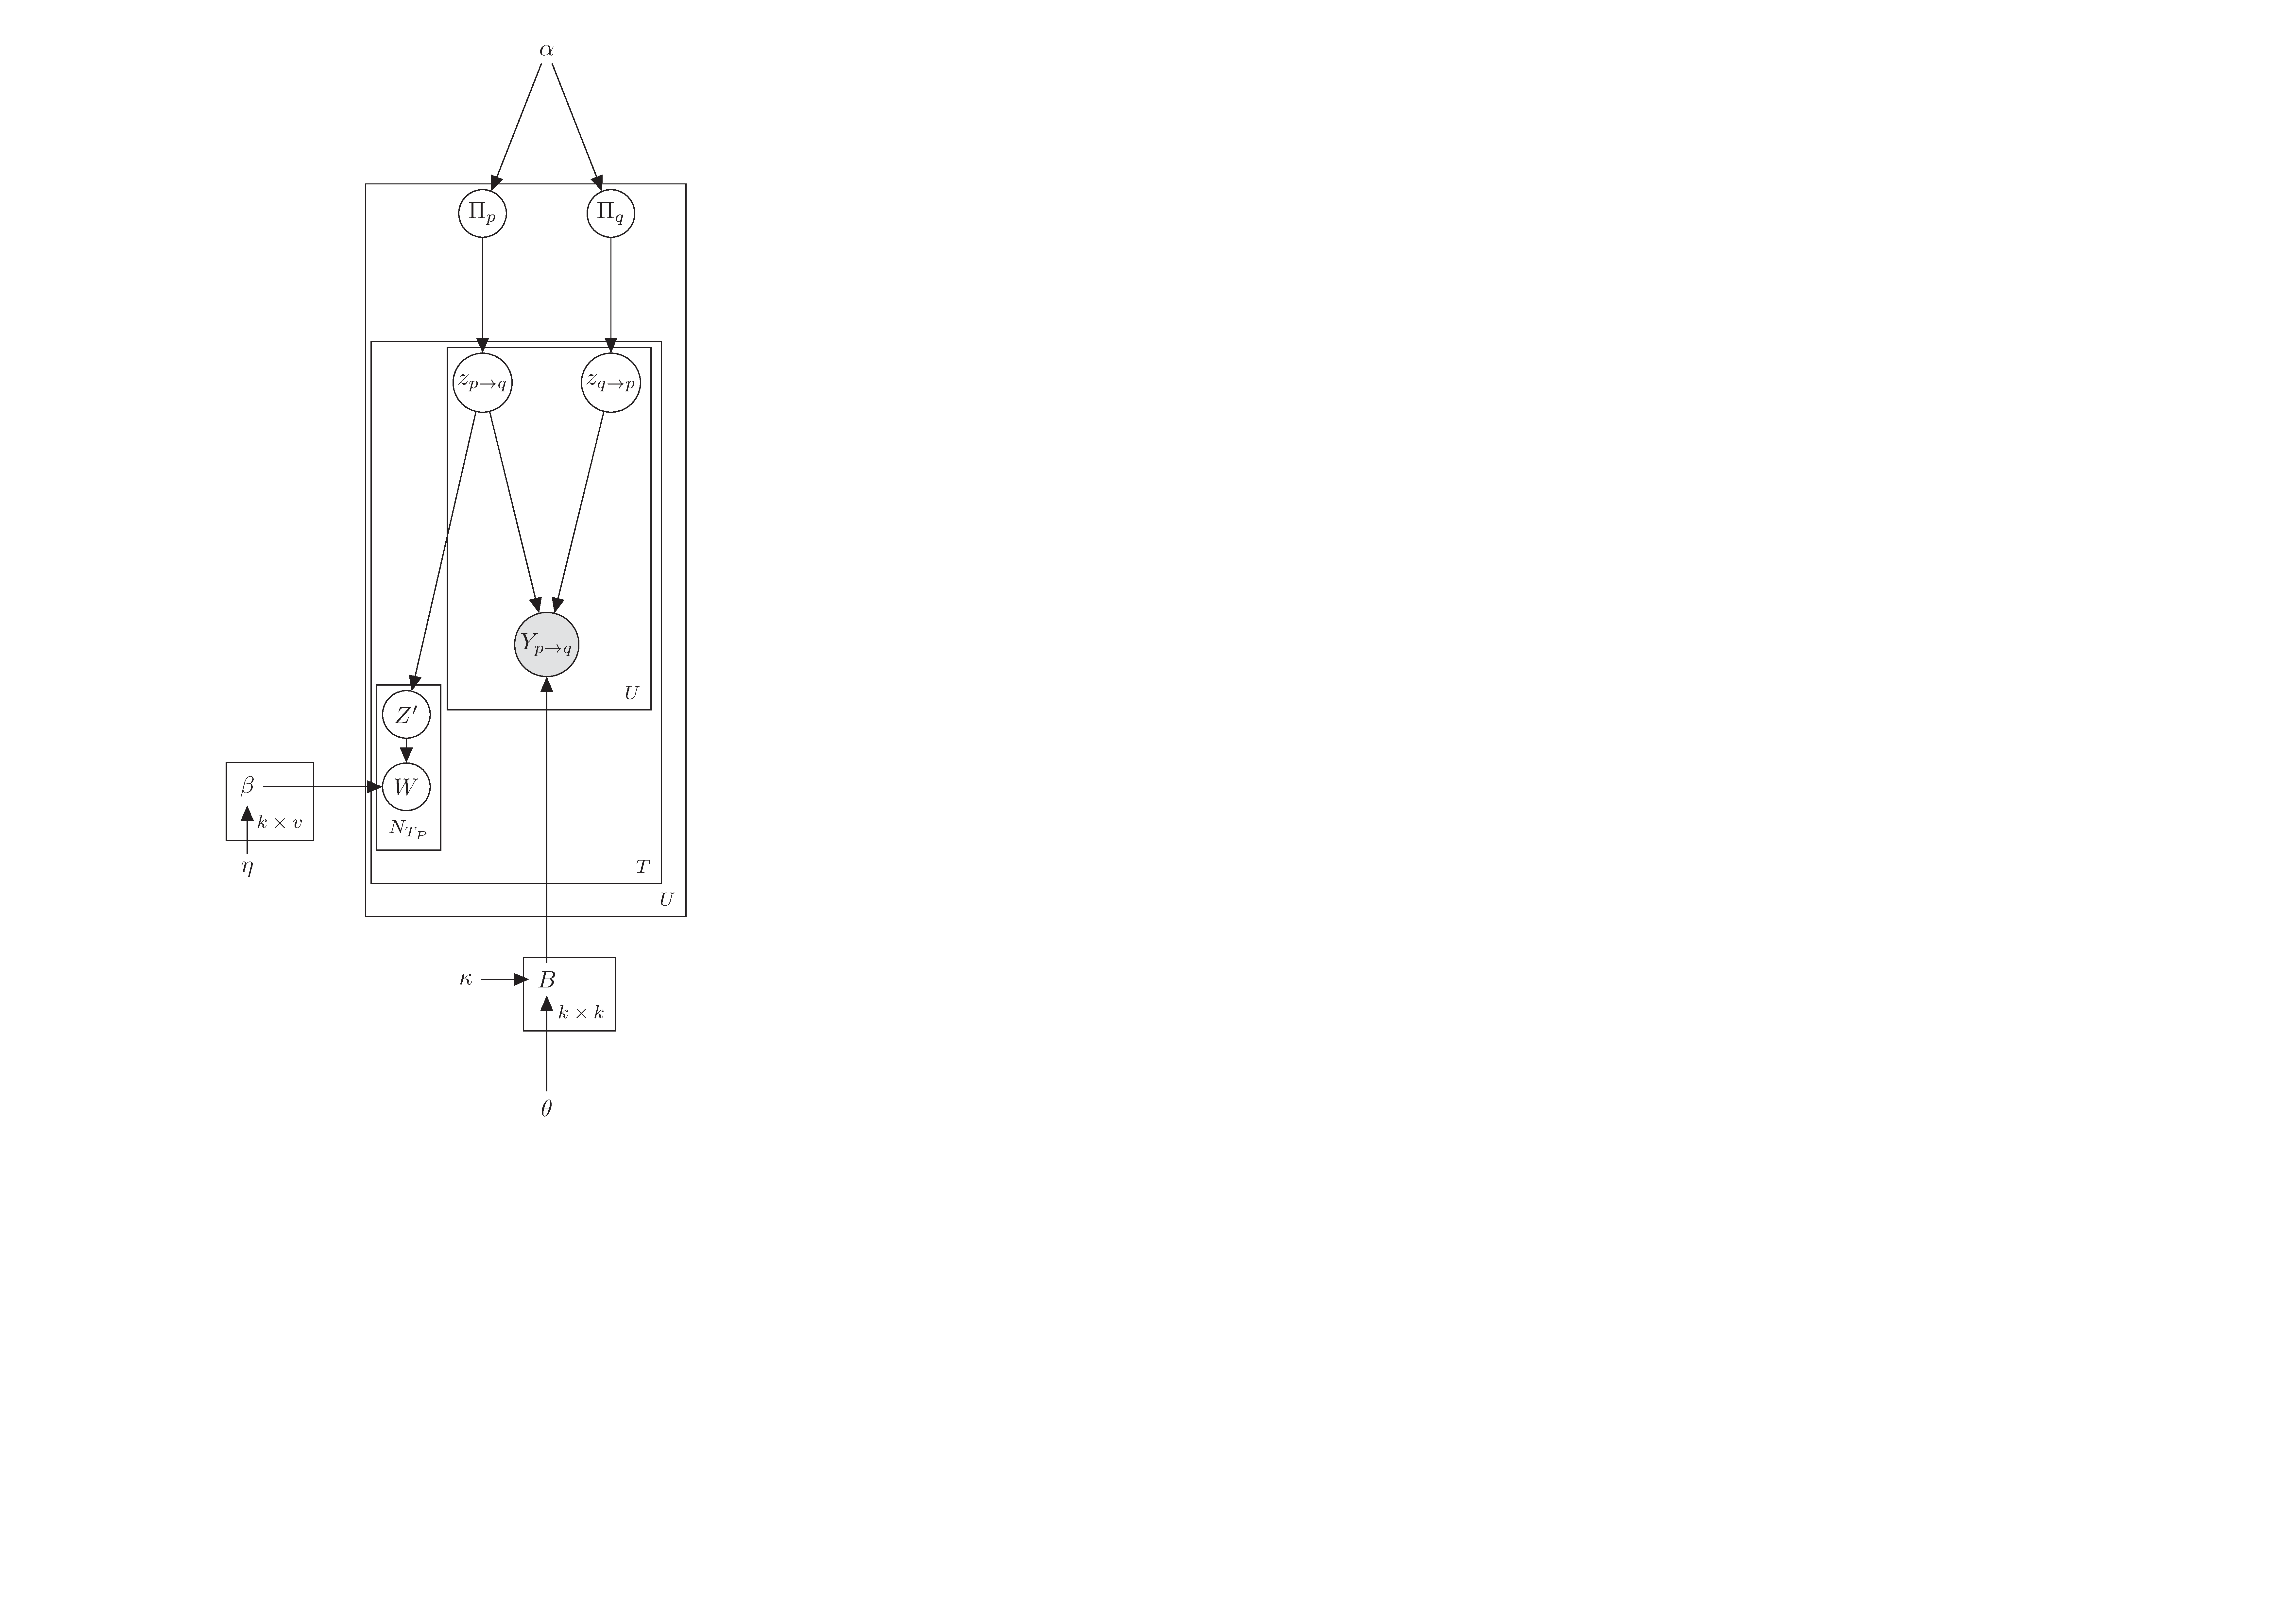
\includegraphics[height=9cm,width=7cm]{pgm_ThreadBased.pdf}
\caption{The proposed approach models active sub-network of users in the forum.
Parameter $T$ determines the number of such sub-networks.
}
\label{fig:finalThreadAggregationModel}
\end{figure}

%Assuming that there are total $N_t$ users in the thread $t$.  
\begin{itemize}
  \item For each Thread $t$
\begin{itemize}
  \item For each user $p \in$ thread $t$
  \begin{itemize}
    \item Draw a $K$ dimensional mixed membership vector 
    $\overset{\rightarrow}{\uppi}_{p} \sim$ Dirichlet($\alpha$)

    \item Draw $B(g,h) \sim Gamma(\kappa,\eta)$; where $\kappa, \eta$ are
    parameters of the gamma distribution.
  \end{itemize}

  \item For each pair of users $(p, q)$ and each thread $t$:
  \begin{itemize}
    \item Draw membership indicator for the initiator, 
    $\overset{\rightarrow}{z}_{(p \rightarrow q,t)} \sim$
    Multinomial($\uppi_{p}$).
    \item Draw membership indicator for the receiver,
    $\overset{\rightarrow}{z}_{(q \rightarrow p,t)} \sim$
    Multinomial($\uppi_{q}$).
    \item Sample the value of their interaction, $Y(p,q,t) \sim$
    Poisson(${\overset{\rightarrow}{z}}^{\top}_{(p \rightarrow q,t)}
    B~\overset{\rightarrow}{z}_{(p \leftarrow q,t)}$). 
	\end{itemize}
	\item For each user $p \in t$
	\begin{itemize}
	  \item Draw $z^{'}_{t,p,k}$ from $Dirichlet(\beta)$.
	  \item Form the set $\delta_{t,p}$ that contains all the users that p
	  interacts to on thread $t$
	  \begin{itemize}
	    \item For each word $w \in N_{t,p}$ 
	    \item Draw $w \sim \phi(w|\sum_{\forall q\in \delta_{t,p}} z_{(t,p
	    \rightarrow q)}) $
	  \end{itemize}
  \end{itemize}
\end{itemize}  
\end{itemize}

The use of Poisson distribution for $Y(p,q,t) \sim$ \\
    Poisson(${\overset{\rightarrow}{z}}^{\top}_{(p
\rightarrow q,t)} B~\overset{\rightarrow}{z}_{(p \leftarrow q,t)}$) (the 
network edge between the user's $p$ and $q$) besides modelling non-binary edge
strength enables the model to ignore non-edges between users ($Y_{t,p,q}$) and
thus faster convergence. In MMSB style community block models non-edges are to be modelled
explicitly.
\begin{equation}
%\begin{align}
\log L = \log \! P(Y, W, Z_{\leftarrow}, 
Z_{\rightarrow}, \Pi, B, \beta | \alpha, \eta, \theta, \alpha) \\
%      &= \sum_{t} \bigg[ \sum_{p,q} \! \log P(Y_{t,p, q} | Z_{t,p \rightarrow q} 
%      , Z_{t,p \leftarrow q}, B) \\ \nonumber 
%      &+ \sum_{p,q} \log P(Z_{t, p \rightarrow q} | \Pi_q) \\ \nonumber 
%      & + \sum_{p,q} \log \! P(Z_{t, p \leftarrow q} | \Pi_{q}) \bigg] 
%      + \sum_{p} \log \! P(\Pi_{p} | \alpha)  \\ \nonumber 
%      & + \bigg[ \sum_{t=1}^{T} \! \sum_{p \in t} \sum_{i=1}^{N_{T_{p}}} 
%      \log \! P(w_{t,p,i} | Z'_{t,p,i}, \beta) \\ \nonumber 
%      & + \sum_{t=1}^{T} \sum_{p \in t} \sum_{i=1^{N_{T_{p}}}} \log \! 
%      P(Z'_{t,p,i} | \bar{Z}_{t, p \rightarrow q}) \bigg] + \sum_{k} \log P(\beta_{k} | 
%      \eta)  
%      \\ \nonumber & +  \sum_{g,h} \log P(B_{g,h} | \kappa, \theta)\\ \nonumber
% \label{eqn:LL}
%\end{align}
\end{equation}
The log-likelihood of the model described in \ref{sec:gen-story} is given
 above and derived in detail in the appendix ~\ref{eqn:LL}.

\begin{align}
q = &\prod_{p}q(\Pi_{q} | \gamma_{p}) \prod_{t} \bigg[ \prod_{p, q} \! 
q(Z_{t, p \rightarrow q}, Z_{t, p \leftarrow q} | \phi_{t,p,q})  \nonumber\\ 
\cdot &\prod_{p \in t} \prod_{i=1}^{N_{T_{p}}} q(Z'_{t,p,i} | \chi_{t,p,i})
\bigg] \nonumber \\
\cdot & \prod_{g,h} q(B_{g,h} | \nu_{g,h} \lambda_{g,h}) \prod_{k} q(\beta{k} | \tau_{k})
\label{eqn:variationalQ}
\end{align}
We use variational approximation to maximize log-likelihood.
Equation~\ref{eqn:variationalQ} above is the approximation of the log-likelihood and we
use structured mean field~\cite{Xing_et_al:2003} to maximize parameters of $q$.
The local variational parameters, $\phi$ (MMSB parameters) and $\chi$ (LDA)
parameters, are maximized using equations \ref{eqn:phiUp} and \ref{eqn:chiUp}
where $\Delta_{\phi^{'}_{t,p,g,h}}$ and $\Delta_{\chi^{'}_{t,p,g,h}}$ are
defined by equations ~\ref{eqn:phiDelta} and~\ref{eqn:chiDelta} respectively.

\begin{align}
\phi_{t,p,g,h} \propto e^{\Delta_{\phi^{'}_{t,p,g,h}}}
\label{eqn:phiUp}
\end{align}



\begin{align}
\chi_{t,p,i,k} \propto e^{\Delta_{\chi^{'}_{t,p,g,h}}}
\label{eqn:chiUp}
\end{align}

The traditional variational updates for global parameters $\gamma, \nu, \lambda$
(MMSB) and $\tau$ (LDA) are defined using equations
\ref{eqn:gammaUp}, \ref{eqn:nuUp}, \ref{eqn:lambdaUp} and \ref{eqn:tauUp}
respectively (details are in the appendix~\ref{sec:appendix}).
% ~\ref{sec:appendix}.



\section{Scalable Estimation}
\label{estimation}

\begin{figure}
\begin{center}
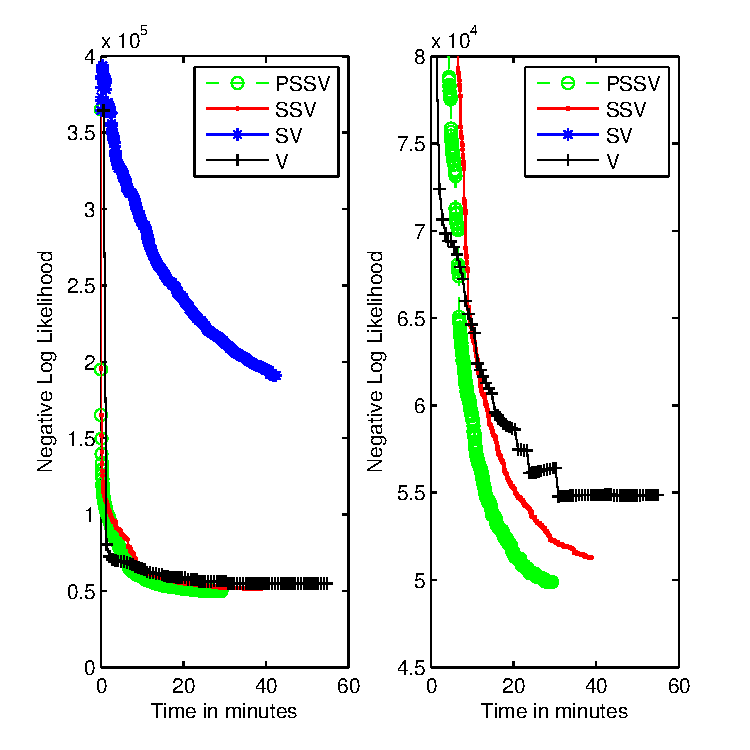
\includegraphics[height=6cm,width=9cm]{SpeedOptimization.pdf}
\end{center}
\caption{The log-likelihood vs incremental speed optimization routine
additions. The right hand plot is a zoomed in version of the left.}
\label{fig:SpeedOptimization}
\end{figure}
The global update equations in previous sections are computationally
very expensive and slow as we need to sum over all the updated local
variables. $N$ users with $T$ threads and vocabulary size $V$ leads to
$O(N^2T+NVT)$ local variables. Traditional sampling or 
variational estimation techniques would be
quite slow for such a model. In order to obtain faster convergence we
make use of stochastic variational approximation along with
sub-sampling and parallelization. 
% Algorithm~\ref{algo:stochasticAlgo} describes in detail the sub-sampled SVI
% based approximate estimation of the model. 

The updates in case of SVI with sub-sampling follow a two step procedure. Step
one computes a local update for the global variables based on the sub-sampled
updated local variables. The local updates ($\gamma^{'},
\nu^{'}, \lambda^{'}$ and $\tau^{'}$) for the global variables ($\gamma,
\nu, \lambda$ and $\tau$) are 

\begin{align}
\gamma_{p,k}^{'} &= \alpha_{k} + \frac{NT}{2|S_p|}\sum_{q \in S_p} \sum_{h}
\! \phi_{t,p,q,k,h} + \frac{NT}{2|S_p|}\sum_{q \in S_p} \! \sum_{g} \!
\phi_{t,q,p,g,k} 
\label{eqn:gammaUpStoc}
\end{align}
  

\begin{align}
\nu_{g,h}^{'} &= \nu_{g,h}^{t}+\rho_\nu \frac{NT}{2|S_p|}\sum_{q \in
S_p}\frac{dL}{\partial\nu_{g,h}}
\label{eqn:nuUpStoc}
\end{align}

\begin{align}
\lambda_{g,h}^{'} &= \frac{\bigg( \sum_{t} \! \sum_{p,q} \! \phi_{t,p,q,g,h}
y_{t,p,q} + \kappa_{g,h} \bigg) }{
 \bigg( \bigg( \sum_{t} \! \sum_{p,q} \! \phi_{t,p,q,g,h} \bigg) + 
\frac{1}{\theta_{g,h}} \bigg) \nu_{g,h}}
\label{eqn:lambdaUpStoc}
\end{align}

\begin{align}
\tau_{p,v}^{'} = \nu_{v} + \frac{NT}{2|S_p|} 
\bigg(\sum_{w_{t,p,i}=v}^{N_{t,p}} \chi_{t,p,i,k} \bigg) 
\label{eqn:tauUpStoc}
\end{align} 

\IncMargin{1em}
\begin{algorithm}[t]
\small
\SetAlgoLined
Input : $Y,W,P,\alpha,\theta,\kappa,\eta$\\
Initialize : $\gamma\leftarrow \gamma_0$,
$\tau\leftarrow \tau_0, \nu\leftarrow \nu_0, \lambda\leftarrow \lambda_0$\\
\While{not converged}{
\For{$c$ processors \textbf{in parallel}}{
	pick a set of threads $T$
	\For{each $t\in T$}{ 	
		pick a node $p$, $\forall q\in~neighborhood~\delta_{t,p}$\\
		\While{$\phi~\&~\chi$ not converged}{
			get new $\phi_{t,p\rightarrow q}$, $\phi_{t,p\leftarrow q}$,
			$\phi_{t,q\rightarrow p}$, $\phi_{t,q\leftarrow p}$\\
			and $\chi_{t,p,i} \forall i \in N_{t,p}$ \\
			iterate between $\phi$ and $\chi$ using
			equations~\ref{eqn:phiUp}~and~\ref{eqn:chiUp}			
			}
		}
	}
aggregate $\phi$ and $\chi$ obtained from different processors.\\
get local update $\gamma^{'}$,$\tau^{'}$, $\nu^{'}$, $\lambda^{'}$ via
stochastic approximation of
equations~\ref{eqn:gammaUp},\ref{eqn:tauUp},\ref{eqn:nuUp},\ref{eqn:lambdaUp}.\\
get global updates of $\gamma$,$\tau$, $\nu$, $\lambda$; e.g. $\gamma^{t+1} =
(1-step)\gamma^{t}+(step)\gamma^{'}$ \\
Similarly globally update $\tau,\nu,\lambda$ as above using
equation~\ref{eqn:globalUpStoc}.
}
\label{algo:stochasticAlgo}
\caption{PSSV: Parallel Sub-sampling based Stochastic Variational inference for
the proposed model}
\end{algorithm}




where $S_p$ is a set of neighborhood edges of user $p$, and $N$ and $T$ are
total number of edges and threads respectively in the network. The set $S_p$ is
chosen amongst the neighbors of $p$ by sampling equal no. zero and non-zero
edges. 

In step two of the sub-sampled SVI the final update of global variable is
computed by the weighted average of the local updates of the global variable and
the variables value in the previous iteration:

\begin{align}
\mu^{t+1} = (1-\omega)\mu^{t} + \omega\mu^{'} 
\label{eqn:globalUpStoc}
\end{align} 

where $\mu$ represents any global variable from $\lambda, \nu, \gamma, \tau$.
the $\omega$ is chosen appropriately using SGD literature and is
decreasing~\cite{conf/nips/GopalanMGFB12}. Tuning $\omega$ is done over
the heldout set described in section~\ref{sec:setup}.
We achieve further speed by parallelizing the text ($\chi$) and network
($\phi$) local variational updates. This is achievable  as the
dependency between $phi$ and $\chi$ parameters allows us to parallelize their
variational updates. Algorithm~\ref{algo:stochasticAlgo} describes the
parallelized SVI updates for the local parameters.


Figure~\ref{fig:SpeedOptimization} 
shows a plot of how the final (p)arallel (s)ub-sampling based (s)tochastic
(v)ariational (PSSV) inference is faster than each of its individual components.
The graph is full run over the SO dataset described in section~\ref{sec:dataset}.
The number of parallel threads in the PSSV scheme is 4. The amount of
sub-sampled forum threads is 400 and the total number of threads is 14,416.
All the schemes in the graph start with the same initialization values of the
hyper-parameters. PSSV is atleast twice as fast as the nearest scheme besides
obtaining the best log-likelihood of all the four at the point of convergence.
The SV (stochastic variational) samples one thread at a time and due to that
takes some time in the beginning to start minimizing the objective value. The
objective value increases in the first few iterations. The number of iterations
to be done by SV is very large but each iterations takes the smallest time of
all 4. The V (variational) scheme takes the least number of iterations to
converge though its iterations are the most time consuming as it has to go
through all the 14,416 threads in every iteration. 
\begin{table}
\begin{center}
\begin{tabular}{c|c|c|c|c|}
 & users & threads & posts & edges\\\hline
 TS & 22,095 & 14,416 & 1,109,125 & 287,808\\\hline
 UM & 15,111 & 12,440 & 381,199 & 177,336\\\hline
 SO & 1,135,996 & 4,552,367 & 9,230,127 & 9,185,650\\\hline
\end{tabular}
\label{tab:dataStats}
\end{center}
\caption{Dataset statistics. SO mostly has edges with weight one.}
\end{table}

\section{Datasets}
\label{sec:dataset}

\begin{figure}
\begin{center}
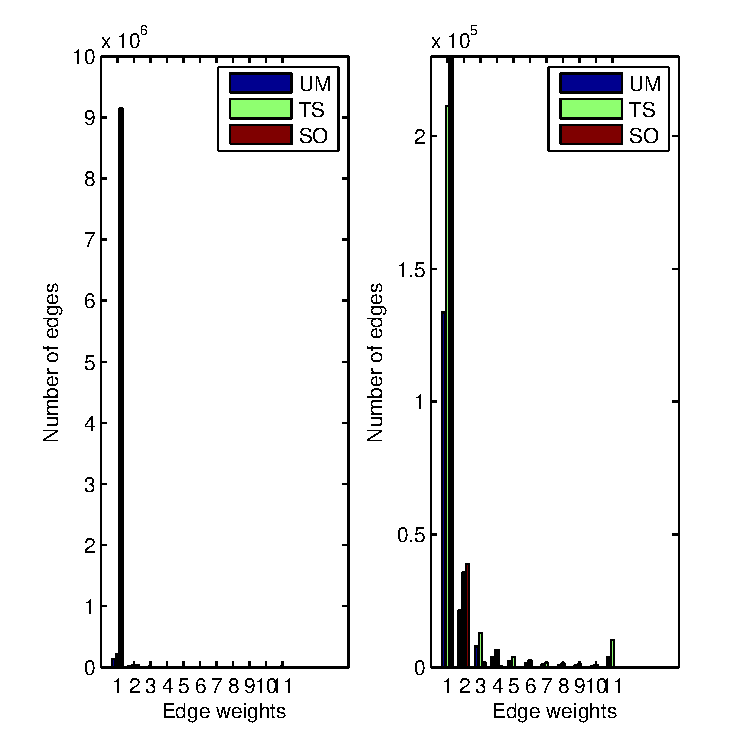
\includegraphics[height=6cm,width=9cm]{EdgeDistribution.pdf}
\end{center}
\caption{Distribution of different edge weights over the 3 datasets. SO 
predominantly consists of edges with weight one. Right hand plot is a scaled
version of the left. The label '11' contains edges weights of 11 and above.}
\label{fig:EdgeDistribution}
\end{figure}

We analyse three real world datasets corresponding to two different forums: 1)
Cancer-ThreadStarter, 2) Cancer-UserName, and 3) Stack Overflow. To test the
stability of the model we use a synthetically generated dataset. 
The Cancer forum is an online breast cancer self-help
community\footnote{\url{http://community.breastcancer.org}} where users
diagnosed with cancer or concerned individuals discuss treatments, their
specific situation besides networking and socializing. StackOverflow is an
online forum for question answering primarily related to computer science. We
use the latest dump of Stack
Overflow~\footnote{\url{http://www.clearbits.net/torrents/2141-jun-2013}}. In
each of these datasets a user posts multiple times in a thread and all these
posts are aggregated into one bigger posts per thread as defined in
section~\ref{sec:gen-story}.
Number of times a user $u$ replies to user $v$ in thread $T$ is the edge weight
of edge $u\rightarrow v$ in thread $T$.

\subsection{Cancer-ThreadStarter (TS)}
In Cancer forum, the conversations happen
in a structured way where users post their responses on a thread by thread
basis. Every thread has a thread starter that posts the first message and
starts the conversation. We build a ThreadStarter graph using this phenomena
where in there is an edge to the thread starter from any user that posts on that
thread. This graph has 22,095 users and 14,416 Threads. 
% \comment{Put number of
% posts and edges}
\subsection{Cancer-Username Mention (UM)}
Users call each other by their usernames (or handle assigned to them in the
forum) while posting in many cases. We create a graph where in an edge between
user $u$ and user $v$ in thread $t$ means that user $u$ calls user $v$ by
username in thread $t$. This forum has 15,111 users and
12,440 threads.
% \comment{Put number of posts and edges}

\subsection{Stack Overflow (SO)}
In Stack Overflow users ask questions and then other users reply with their
answers. We obtain the ThreadStarter graph from this structure. This dataset has
have 1,135,996 users and 4,552,367 threads.
% \comment{Put number of posts and edges}
Table~\ref{tab:dataStats} gives the distributions of edges, posts, users and
threads in the three datasets used. 
\subsection{Synthetic data}
We generate a synthetic dataset using the generative process defined in
section~\ref{sec:gen-story}. We have 1000 users and 100 threads. 
\comment{Put number of posts and edges as well as the parameters}
\\
 
\begin{figure}
\begin{center}
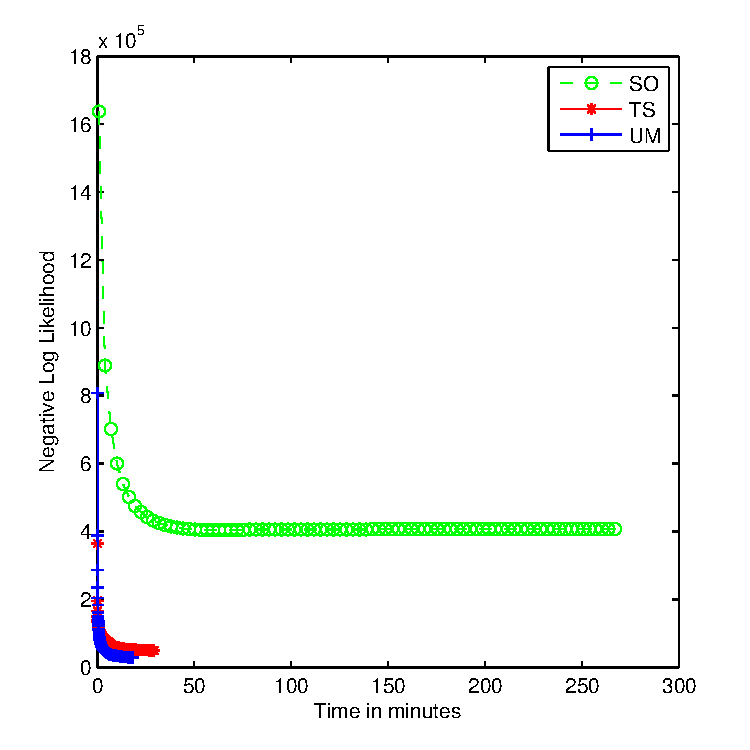
\includegraphics[height=6cm,width=9cm]{3LLPlots.pdf}
\end{center}
\caption{The log-likelihood over heldout set for the fully tuned model on the
3 datsets}
\label{fig:finalLLheld}
\end{figure}
 
\section{Experimental Setup and Evaluation}
\label{sec:setup}
We divide each of our datasets into three sets: 1) training set, 2) heldout set,
and 3) test set. We learn our model on training set and tune our hyperparameters
($\alpha, \eta, \kappa, \theta$ etc.) on heldout set. The split is done over the
edges where 80\% of the edges are in training and rest 20\% are divided amongst
heldout and test equally. 
For the two Cancer datasets we only predict non-zero edge weights whereas for
the Stack Overflow we predict edges that are absent as well as those that are
present with their corresponding edge weights. Graph
\ref{fig:EdgeDistribution} shows the distribution of edge weights in
cancer as well as Stack Overflow dataset. We chose Stack Overflow to predict
zero weights since it has predominantly edges with very low weights,
predominantly weight of one. This demonstrates that the model is versatile. In
addition to 20\% of the total non-zero edges we randomly sample equal
number of zero edges from the graph for the SO held and test set. 
The optimization objective for learning is defined in
equation~\ref{eqn:VarLowerBound}.
\paragraph{Link-prediction} We predict the edge-weight of the edges present in
the test set. The predicted edge, $\hat{Y}_{t,u,v}$, between users $u$ and
$v$ in thread $t$ is  defined as 
\begin{align}
\hat{Y}_{t,u,v} = \pi^T_uB\pi_v\label{eqn:prediction}\\
B=\nu.*\lambda\label{eqn:blockMat}
\end{align}
and the prediction error is the $rmse$, defined as given predicted edge
$\hat{Y}_{t,u,v}$ and the actual edge $Y_{t,u,v}$,
\begin{equation}
rmse=\sqrt{\sum(\hat{Y}_{t,u,v}-Y_{t,u,v})^2}
\end{equation}

\begin{figure}
\begin{center}
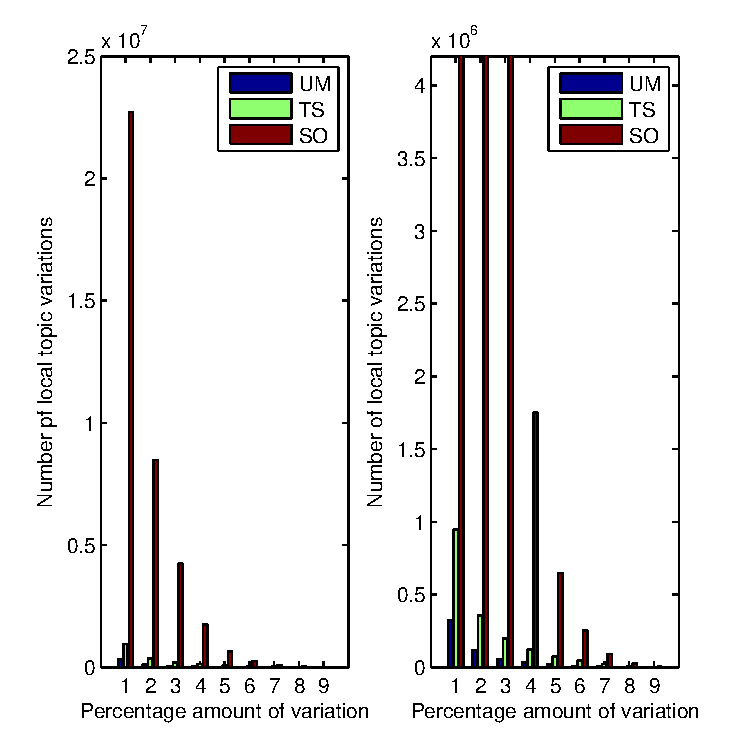
\includegraphics[height=6cm,width=9cm]{TopicVariationsLocal.pdf}
\end{center}
\caption{Number of local variations in topic proportion on a per user per thread
level. The right hand plot is a scaled in version of the left.}
\label{fig:localTopicVariations}
\end{figure}

The summation is over the edges in the test (or heldout) set. The block matrix
$B$ described in equation~\ref{eqn:blockMat} is well defined for both MMSB the proposed
model. Hence the prediction is obtained for the active network modelling without
LDA (just MMSB component) and with LDA. We created an artificial
weighted Identity matrix for LDA $\hat{B}=m*I$. It is a diagonal matrix with
all element values $m$. For every user $u$ and every thread $t$ the topics discovered over the
posts of $u$ in $t$ is used as the vector $\pi_u$ in
equation~\ref{eqn:prediction} for prediction. A diagonal $B$ is desirable in
block models as it provides clean separation among the clusters
obtained~\cite{Airoldi:2008:MMS:1390681.1442798}.
The value of $m$ is tuned over heldout set. We define a basic baseline that
always predicts the average weight ($\bar{Y}$) all the edges, zero (Stack
Overflow) or non-zero (Cancer), in the heldout or test set.
\begin{equation}
rmse_{baseline} = \sqrt{\sum(\bar{Y}-Y_{t,u,v})^2}
\end{equation}
\begin{center}
\begin{figure*}
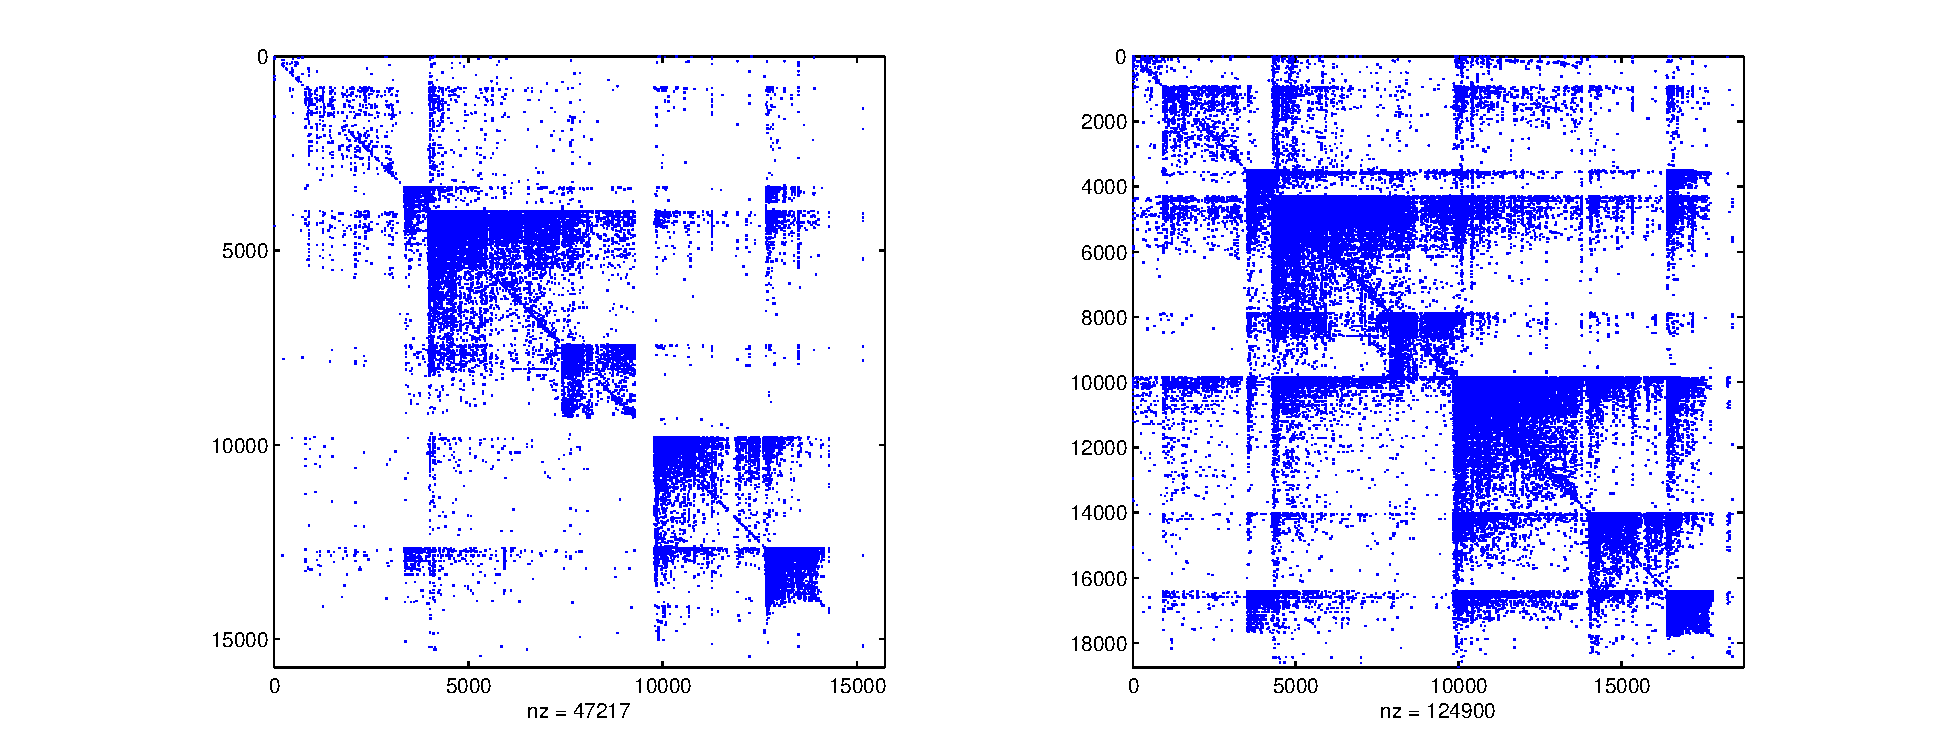
\includegraphics[height=7cm,width=18cm]{SimilarityMatTS.pdf}
\caption{Similarity Matrix of the users clustered by MMSB(left) and our model
(right) using their dominant role as cluster index over TS dataset. Our model
assigns 3K more users that MMSB discards and discovers a new cluster (2nd block
from bottom to top along the main diagonal)}
\label{fig:similarityMatTS}
\end{figure*}
\end{center}

\paragraph{Parameter tuning}
Figure~\ref{fig:finalLLheld} shows plot of tuned log-likelihood over the 3
datasets against time. UM being the smallest of the two takes
the least amount of time. \comment{A big graph for: choosing the number of
topics, choosing the hyperParameterss,choosing the $S_p$ for the sub-sampling of
the edges in the user neighborhood, Choosing the balancing factor between the
text and the network}\\

\section{Results}
\paragraph{Link prediction} Table~\ref{tab:predictionResults} shows the link
prediction results on heldout and test set for the for the four prediction
model.
\begin{table}
\begin{center} 
\begin{tabular}{p{1cm}|p{0.7cm}|p{0.7cm}|p{0.7cm}|p{0.7cm}|p{0.7cm}|p{0.7cm}|}
  & UM held & UM test & TS held & TS test & SO held & SO test \\\hline
Our Model & \textbf{1.303} &\textbf{1.292} &\textbf{2.782} & \textbf{2.748} & 
\textbf{0.348}& \textbf{0.361} \\\hline 
MMSB &1.450& 1.502 & 2.984& 2.881 &0.421 & 0.434 \\\hline 
LDA &1.793& 1.731	&3.725 & 3.762 &0.466 & 0.479\\\hline
Baseline &1.886& 1.983 &4.504 &4.417&0.502& 0.509\\\hline
\end{tabular}
\caption{Link prediction results over the 3 datsets }
\label{tab:predictionResults}
\end{center}
\end{table}

The proposed approach to model thread level conversational roles outperforms
all of the other models. LDA performs poorer than MMSB since LDA does not 
explicitly model network information. 
\paragraph{Cancer dataset}
Figure~\ref{fig:localTopicVariations} shows the number of times the global role
of a user is different from the thread level role that he plays. It is very
interesting to see that the variations between global and thread level role
assignment are a lot. A model that ignores this local vs global dynamics tends
to lose a lot of information. Figure~\ref{fig:similarityMatTS} shows the plot of
the user by user similarity matrix obtained from our model vs MMSB model for TS
dataset.
We take all users and assign them the cluster that they have more than 50\% of
chance of lying in. If a user doesn't have such a dominant topic then he is
discarded. Our model is unable to assign a clear role to 3.3 K users and
the MMSB approximately to 6.3K users out of 22K. As seen in the figure,
the combined model is able to effectively find the main roles for the extra 3K users that the
MMSB model was unable to provide for effectively. The clusters also look a lot
denser for the proposed model. A new cluster block that is not
accounted for by MMSB is discovered by the proposed model
(figure~\ref{fig:similarityMatTS}).

 \comment{Put interpretations of the clusters, UserName and
ThreadStarter}\\
\comment{Put the top 10 words in each topics}\\
\comment{Put Block matrix to demonstrate better resolution of cluster}\\
\comment{Put nice visualization for some per user-thread topic proportions.}\\
\paragraph{Stack Overflow} 
\comment{Put interpretations of the clusters}\\
\comment{Put the top 10 words in each topics}\\
\comment{Put Block matrix to demonstrate better resolution of cluster}\\
\comment{Put nice visualization for some per user-thread topic proportions.}\\
\paragraph{Synthetic dataset}
\comment{provide plots of rmse between the inferred and the actual
parameters, $\pi$ over random runs of the model }\\
% \subsection{Cluster Interpretations}
% 
% \subsection{Link prediction}
% We hold out some users randomly in the dataset and predict their
% likelihood of interaction with other users based solely on the content of their
% posts in the forum and the parameters of the model learnt in the training phase. 
% We take the top K (1, 5 and 10) users that the model predicts for every held-out
% user and report the overall precision and recall in the top-K set. This will
% have to be done for a specific snapshot of the forum because not many users will
% have a overlapping posting history accross their whole stay on the forum.
% 
% \subsection{Cancer forum user survival prediction}
% Users in cancer forum posts different messages at different phases of theor
% cancer. It has been seen that in while users are certain cancer phase they tend
% to post more often and regularly. The intuition behind this prediction task is
% to exploit this pattern. We use the variational parameter of the
% $\bar{Z_{p\rightarrow}}$ to get the topic composition of a users posts in the
% forum at one particular snapshot of time e.g. every month or every two months.
% We combine the features shown to be useful for such an analysis by Wen et
% al.~\cite{Wen:2013:Carolyn} with the variational parameters to predict whether
% the user will post in the coming period of time e.g. within the next month or
% two months.
% 
% 
% \section{Results}
% \comment{

% Figure~\ref{fig:cancerClusters} shows a set of clusters that we discover over
% Cancer dataset with around 22K users. %\comments{Very preliminary results}
% 
% \begin{figure*}[!tb]
% \centering
% 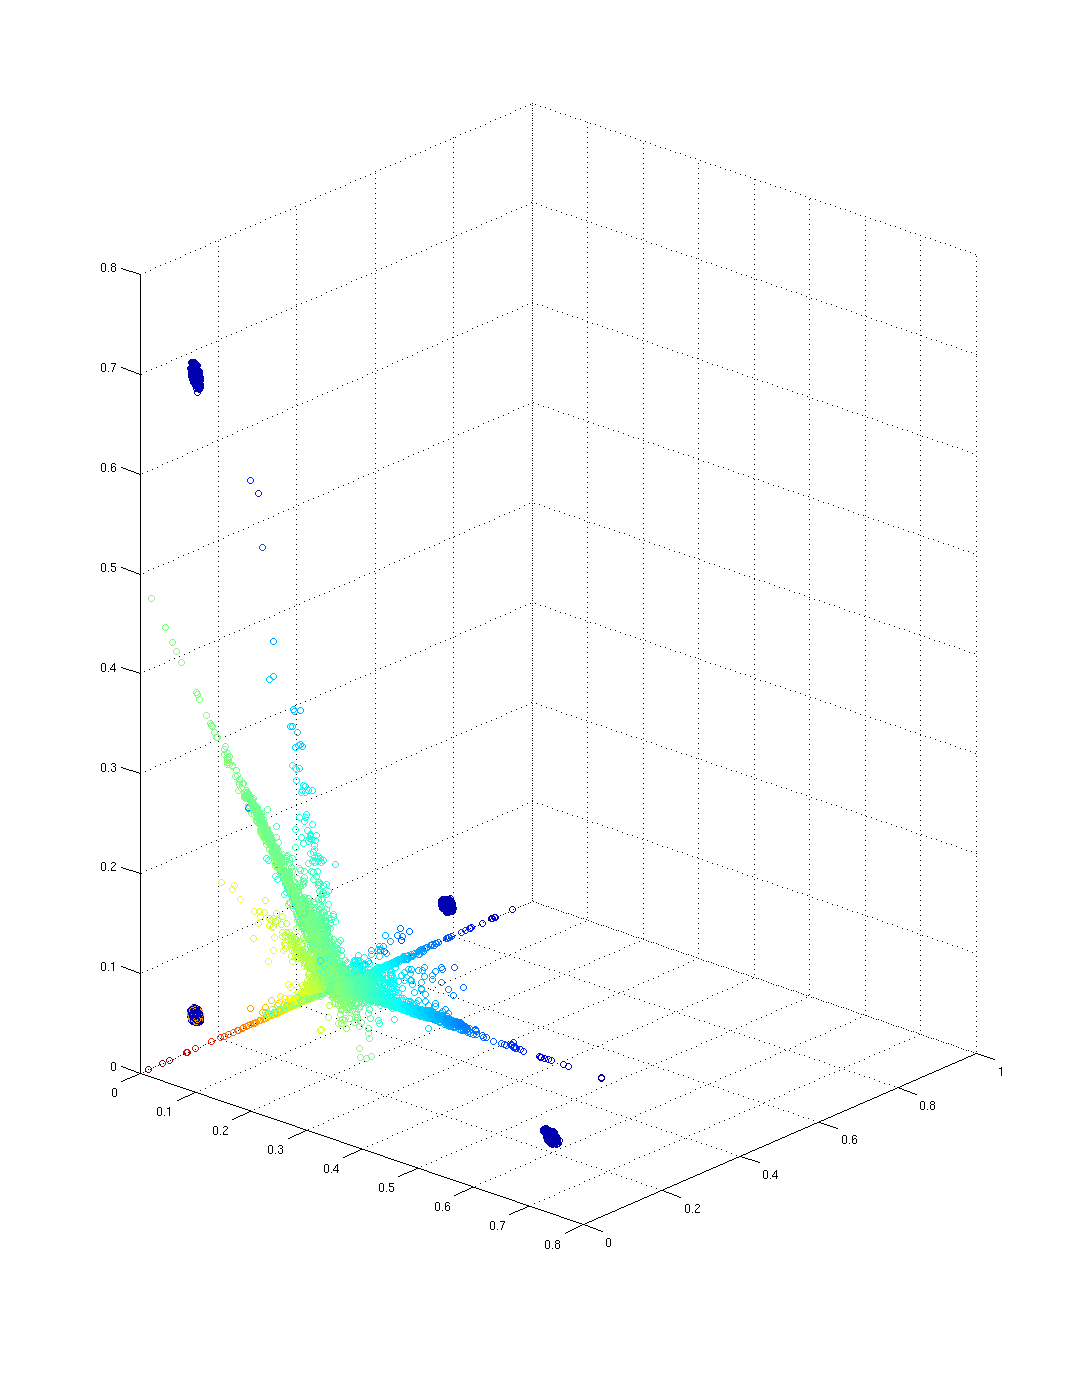
\includegraphics[scale=0.5]{CancerThreadStarter.png}
% \caption{Set of clusters discovered in Cancer dataset}
% \label{fig:cancerClusters}
% \end{figure*}

% Following are the experimemts that we are planning to do\\
% 1. Analyse and interpret the communties discovered on Wikipedia talk pages and
% Cancer forum providing interesting insights and telling how modelling forum
% structure helps. \\
% 2. Validate the above discovered communities either through held out likelihood
% or perplexity. \\ 
% 3. Introduce a prediction task; there were several suggestions: \\
% \hspace{3 cm} a) predict the topic of the posts by a user in a thread where for
% training we have hand-labeled thread posts (suggested by Chong) \\
% \hspace{3 cm} b) Hold out some users on some threads and predict whether the
% user is going to post on the held-out threads \\
% 3. Predicting the popularity of a response/post on Reddit as well as Stack
% Overflow. We can go much finer and predict whether a given user will upvote a
% post or not. We will also have to derive equations for this but shouldn't be
% too hard.
% }



\section{Conclusion \& Future Work}
%  Currently our model just picks up one signal for the network
% component (MMSB part) i.e. in other words we are just modelling one type of
% interaction or just one graph, but as we did for the SEI model (tensor model) 
% there are multiple types of
% networks/graphs/interactions. Future work can incorporate this.\\
% 2) Adding temporal dimension to this model would be a very interesting idea.
% E.g. how threads evolve over time, or how user behavior changes, or how new
% communities emerge in the forum etc.



\bibliography{mybib}
\bibliographystyle{plain}
\appendix
\label{sec:appendix}
% \onecolumn{}

%The log-likelihood of the model:
%\begin{align}
%\log L &= \log \! P(Y, W, Z_{\leftarrow}, 
%Z_{\rightarrow}, \Pi, B, \beta | \alpha, \eta, \theta, \alpha) \nonumber\\
%\nonumber &= \sum_{t} \bigg[ \sum_{p,q} \! \log P(Y_{t,p, q} | Z_{t,p \rightarrow q} 
%     , Z_{t,p \leftarrow q}, B) \\ \nonumber 
%     &+ \sum_{p,q} \log P(Z_{t, p \rightarrow q} | \Pi_q) \\ \nonumber 
%     & + \sum_{p,q} \log \! P(Z_{t, p \leftarrow q} | \Pi_{q}) \bigg] 
%     + \sum_{p} \log \! P(\Pi_{p} | \alpha)  \\ \nonumber 
%     & + \bigg[ \sum_{t=1}^{T} \! \sum_{p \in t} \sum_{i=1}^{N_{T_{p}}} 
%     \log \! P(w_{t,p,i} | Z'_{t,p,i}, \beta) \\ \nonumber 
%     & + \sum_{t=1}^{T} \sum_{p \in t} \sum_{i=1^{N_{T_{p}}}} \log \! 
%     P(Z'_{t,p,i} | \bar{Z}_{t, p \rightarrow q}) \bigg]   
%     \\ \nonumber & + \sum_{k} \log P(\beta_{k} | 
%     \eta) +  \sum_{g,h} \log P(B_{g,h} | \kappa, \theta).\\ 
%     \label{eqn:LL}
%\end{align}

%The data likelihood for the model in figure~1
%
%\begin{align}
%P(Y, R_{p} | \alpha, \beta, \kappa, \eta) &=  \nonumber\\ 
% \int_{\Phi} \!
%\int_{\Pi} \sum_{z} \! P(Y, R_{p}, & z_{p \rightarrow q}, z_{p \leftarrow q},
%\Phi, \Pi | \alpha, \beta, \kappa, \eta)  \nonumber \\  \nonumber
%%\\ 
%= \int_{\Phi} \! \int_{\Pi} \sum_{z} \! \bigg[ \prod_{p,q} & \prod_{t}
%P(Y_{pq}^{t} | z_{p \rightarrow q}^{t}, z_{p \leftarrow q}^{t}, B) 
%\cdot P(z_{p \rightarrow q}^{t} | \Pi_{p}) \nonumber
%\\  \cdot P(z_{p \leftarrow q}^{t} |
%\Pi_{q})   & \cdot \bigg(\prod_{p} P(\Pi_{p} | \alpha) \prod_{t} \prod_{p}
%P(R_{p}^{t} | z_{p \rightarrow q}^{t}, \Phi) \nonumber
%\\ \cdot \prod_{k} P(\Phi_{k} |
%\beta)&\bigg) \cdot \prod_{g,h}P(B_{gh} | \eta, \kappa) \bigg].
%\end{align}

%The complete log likelihood of the model is:
%
%\begin{align}
%\log \! &P(Y, W, z_{\rightarrow}, z_{\leftarrow}, \Phi, \Pi, B | \kappa, \eta,
%\beta, \alpha) \nonumber
%\\ & = \sum_{t} \! \sum_{p,q} \! \log P(Y_{pq}^{t} | z_{p
%\rightarrow q}^{t} , z_{p \leftarrow q}^{t}, B) \nonumber
%\\ &+ \nonumber \sum_{t} \!
%\sum_{p,q} \! (\log P(z_{p \rightarrow q}^{t} | \Pi_{p}) + \log \! P(z_{p \leftarrow q}^{t} |
%\Pi_{p})) \\  
%&+ \sum_{p} \! \log \! P(\Pi_{p} | \alpha) ~+ \sum_{t} \!
%\sum_{p} \! \sum_{w \in R_{p}^{t}} \log P(w | z_{p \rightarrow}, \Phi)
%\nonumber\\ 
%&+ \sum_{k} \! \log P(\Phi_{k} | \beta) + \sum_{gh} \! \log P(B_{gh} | \eta,
%\kappa).
%\end{align}

%The mean field variational approximation for the posterior is 
%
%\begin{align}
%q(z, &\Phi, \Pi, B | \Delta_{z_{\rightarrow}}, \Delta_{\Phi}, \Delta_{B},
%\Delta_{z_{\leftarrow}}, \Delta_{B_{\kappa}})  = \nonumber \\ \prod_{t} \!
%& \prod_{p,q} \! \bigg( q_{1}(z_{p \rightarrow q}^{t} | \Delta_{z_{p \rightarrow
%q}}) + q_{1}(z_{p \leftarrow q}^{t} | \Delta_{z_{p \leftarrow q}})  \bigg) \nonumber \\
%\cdot \prod_{p} &\! q_{4}(\Pi_{p} | \Delta_{\Pi_{p}}) \prod_{k} q_{3} (\Phi_{k}
%| \Delta_{\Phi_{k}}) \prod_{g,h} \! q(B_{g,h} | \Delta_{B_{\eta}},
%\Delta_{B_{\kappa}}).
%\end{align}

The lower bound for the data log-likelihood from jensen's inequality is: 

\begin{align}
&L_{\Delta} = E_{q}\bigg[ \log \! P(Y, W, z_{\rightarrow}, z_{\leftarrow}, \Phi,
\Pi, B | \kappa, \eta, \beta, \alpha) - \log \! q \bigg]\nonumber\\
&= E_{q} \Bigg[ \sum_{t} \! \sum_{p,q} \! \log \left(
B_{g,h}^{Y_{p,q}^t} \frac{e^{-B_{gh}}}{Y_{pq}^{t}!} \right) +
\sum_{t} \! \sum_{pq} \! \log\left( \prod_{k} (\pi_{p,k}^{z_{p \rightarrow q} =
k}) \right) \nonumber\\
&+ \sum_{t} \! \sum_{p,q} \log \! \left(
\prod_{k}(\pi_{q,k})^{z_{p \leftarrow q} = k} \right)\nonumber\\ 
&+\sum_{t} \! \sum_{p} \! \sum_{w\in R_p^t}  \log \! \left(
\prod_{u\in V}(\bar{z}^T\phi_u)^{w = u} \right)
\nonumber\\ &+ 
\sum_{p} \! \log \left( \prod_{k}
(\Pi_{p,k})^{\alpha_{k} - 1} \cdot \frac{\Gamma(\sum \alpha_{k})}{\prod_{k}
\Gamma(\alpha_{k})} \right) \nonumber\\ & + 
\sum_{k} \! \log\left( \prod_{u\in V}
(\phi_{k,u})^{\beta_{k} - 1} \cdot \frac{\Gamma(\sum \beta_{k})}{\prod_{k}
\Gamma(\beta_{k})} \right) \nonumber\\ &+
 \sum_{g,h} \! \log \! \left( B_{g,h}^{\kappa - 1} /
\eta^{\kappa} \Gamma(\kappa) \cdot \exp(-B_{g,h}/\eta) \right) \Bigg]
\nonumber\\ 
& -E_{q} \Bigg[ \sum_{t} \! \sum_{p,q} \log \big( \prod_{k} (\Delta_{z_{p
\rightarrow q}, k})^{z_{p \rightarrow q}=k} \big) \nonumber \\&+ \sum_{t} \!
\sum_{p,q} \! \log \! \left(
\prod_{k} \! (\Delta_{z_{p \leftarrow q}, k})^{z_{p \leftarrow q} = k} \right)
  \nonumber \\
 &+\sum \! \log \left( \prod_{k} \! (\Pi_{p,k})^{\Delta_{\pi_{pk}}-1}
\frac{\Gamma(\Delta_{\Pi_{p}})}{\prod_{k=1} \! \Gamma(\Delta_{\Pi_{p,k}})}
\right) \nonumber \\ &+ 
\sum_{k} \log \! \left( \prod_{u \in v}
(\Phi_{k,u})^{\Delta_{\Phi_{ku}} - 1)} \frac{\Gamma(\Delta_{\Phi_{k}})}
{\prod_{u \in v} \! \Gamma(\Delta_{\Phi_{k,u}})} \right) \nonumber \\ 
&+ \sum_{g,h} \log \! \left(
\frac{B_{g,h}^{\Delta_{\kappa = 1}}}{\Delta_{\eta}^{\Delta_{\kappa}}
\Gamma(\Delta_{\kappa})} \exp(-B_{g,h}/\Delta_{\eta}) \right) \Bigg].
\label{eqn:VarLowerBound}
\end{align}

%$\Delta_{\phi}$ used in the update of $\phi$ in equation~\ref{eqn:phiUp}. The
%parameter $\omega$ is used here to balance out the contribution from the text
%side to the network. 
%
%\begin{align}
%\Delta_{\phi^{'}_{t,p,g,h}} &= y_{t,p,q}( \log \! \lambda_{g,h} + 
%\Psi(\nu_{g,h})) - \nu_{g,h} \lambda_{g,h} - \log \! (y_{t,p,q}!)
%\nonumber \\ & + \Psi(\gamma_{p,g}) - \Psi(\sum_{g} \gamma_{p,g})
%\nonumber \\  & + \Psi(\gamma_{q,h}) - \Psi(\sum_{h} \gamma_{q,h})
%\nonumber \\  & + \omega\sum_{i=1}^{N_{T_{P}}} \! \chi_{t,p,i,g} 
%\bigg[ \ln \! \frac{\epsilon}{\delta_{p,t}} - \frac{1}{\delta_{t,p}} 
%+ \ln \bigg( 1 + \frac{\epsilon}{\delta_{p,t}} \bigg) 
%\cdot \frac{1}{\delta_{t,p}} \bigg].
%\label{eqn:phiDelta}
%\end{align}
%
%$\Delta_{\chi}$ used in equation~\ref{eqn:chiUp} for $\chi$ update
%
%\begin{align}
%\Delta_{\chi^{'}_{t,p,g,h}} &= \bigg[ \Psi(\tau_{k,w_{t,p,i}}) - 
%\Psi(\sum_{w_{t,p,i}} \! \tau_{k, w_{t,p,i}}) \bigg]
%\nonumber \\  & + \ln \! (\frac{\epsilon}{\delta{p,t}}) \frac{1 - 
%\sum_{q,h} \! \phi_{t,p,q,k,j}}{\delta_{t,p}} 
%\nonumber\\  & + \frac{\sum_{q,h} \phi_{t,p,q,k,h}}{\delta_{t,p}} 
%\ln \! (1 + \frac{\epsilon}{\delta_{t,p}}).
%%\nonumber\\  & - 1 - \log \! \chi_{t,p,i,k}
%\label{eqn:chiDelta}
%\end{align}


Partial derivative of $\nu$
\begin{align}
\frac{dL}{\partial\nu_{g,h}} &= \sum_{t} \! \sum_{p,q} \! 
\phi_{t,p,q,g,h} (y_{t,p,q} \Psi'(\nu_{g,h}) - \lambda_{g,h})
\nonumber\\  & + (\kappa_{g,h} - \nu_{g,h})\Psi'(\nu_{g,h}) + 
1 - \frac{\lambda_{g,h}}{\theta_{g,h}}.
\label{eqn:partialNu}
\end{align}

The traditional variational updates for the global parameters

\begin{align}
\gamma_{p,k} &= \alpha_{k} + \sum_{t} \! \sum_{q} \! \sum_{h} \! \phi_{t,p,q,k,h} 
+ \sum_{t} \! \sum_{q} \! \sum_{g} \! \phi_{t,q,p,g,k}.
\label{eqn:gammaUp}
\end{align}

\begin{align}
\nu_{g,h}^{t+1} &= \nu_{g,h}^{t}+\rho_\nu \frac{dL}{\partial\nu_{g,h}}. 
\label{eqn:nuUp}
\end{align}

\begin{align}
\lambda_{g,h} &= \frac{\bigg( \sum_{t} \! \sum_{p,q} \! \phi_{t,p,q,g,h} y_{t,p,q} + 
\kappa_{g,h} \bigg) }{
 \bigg( \bigg( \sum_{t} \! \sum_{p,q} \! \phi_{t,p,q,g,h} \bigg) + 
\frac{1}{\theta_{g,h}} \bigg) \nu_{g,h}}.
\label{eqn:lambdaUp}
\end{align}

\begin{align}
\tau_{p,v} = \nu_{v} + \sum_{t} \! \sum_{p \in t}
\bigg(\sum_{w_{t,p,i}=v}^{N_{t,p}} \chi_{t,p,i,k} \bigg).
\label{eqn:tauUp}
\end{align}


where $\rho_\nu$ is $\nu$'s gradient ascent update step-size using its partial
derivative $\frac{dL}{\partial\nu_{g,h}}$ define in equation~\ref{eqn:partialNu}.



\end{document}
